\section{Introduction}

  A {\it decoration} of the Mandelbrot set $M$ (called also a {\it Misiurewicz limb})
$\LL$ is a part of $M$ cut off by two external rays
 landing at some tip of a satellite copy of $M$ attached to the main cardioid,
see Figure \ref{limbs} (see \S \ref{sec: first king} for the precise dynamical definition).
In this paper we consider infinitely
renormalizable quadratic polynomials satisfying the decoration condition,
which means that the combinatorics of the renormalization operators involved is selected from
a finite family of decorations $\LL_k$. (For instance, real infinitely renormalizable maps
satisfy a decoration condition if and only of non of the renormalizations is of doubling type.)



\begin{figure}
%\centerline{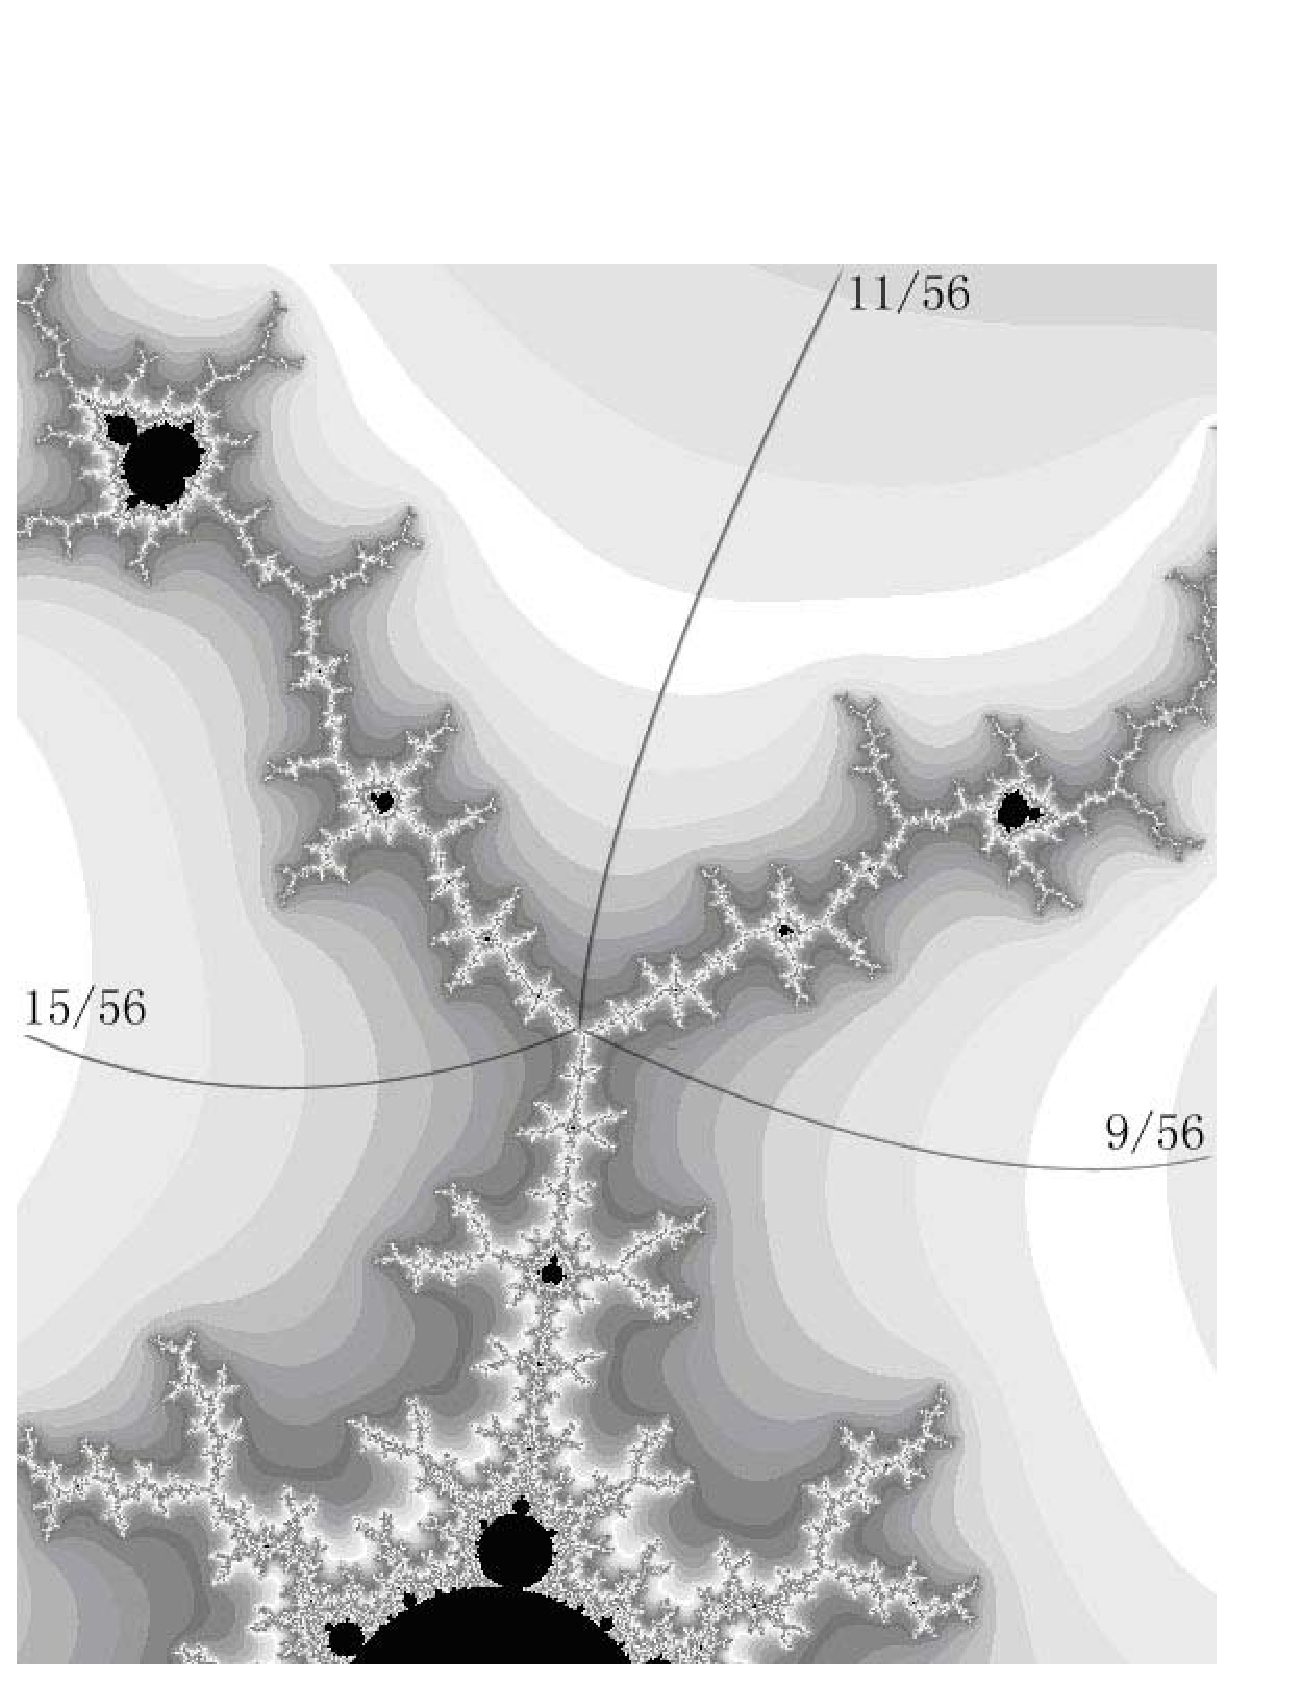
\psfig{figure=limb1.eps,width=.8\hsize}}
\centerline{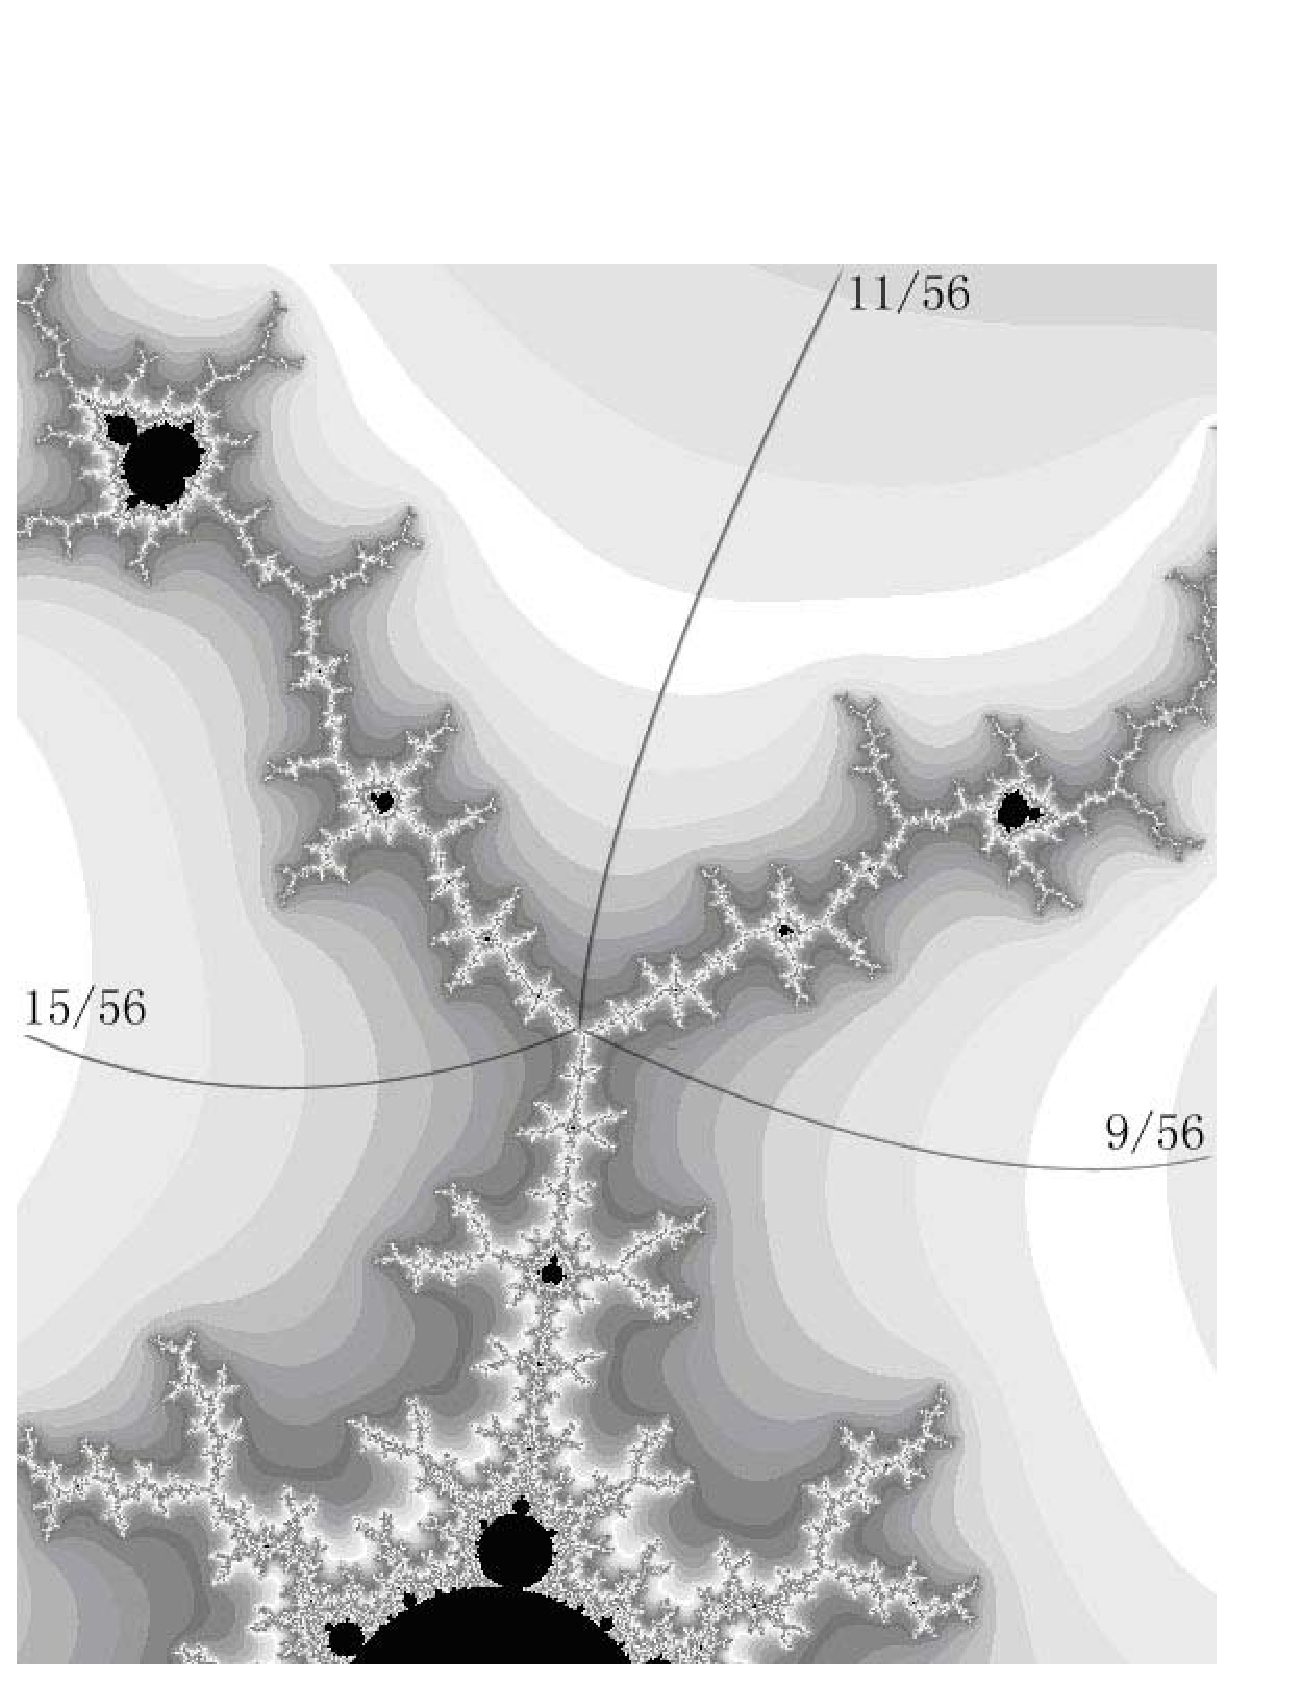
\includegraphics[width=12cm]{limb1.eps}}
\caption{Two decorations of the Mandelbrot set.
   The little Mandelbrot sets inside specify renormalization combinatorics of type $(3,1)$.  \label{limbs}}
 \end{figure}


An infinitely renormalizable quadratic map $f$ is said to have {\it a priori bounds}
if its renormalizations can be  represented by quadratic-like maps  $R^n f: U_n\ra V_n$
with $\mod (V_n\sm U_n)\geq \eps >0$, $n=1,2\dots$.


Our goal is to prove the following result:

\begin{mainthm}
%\proclaim Main Theorem.
  Infinitely renormalizable quadratic maps satisfying the decoration condition have
a priori bounds.
\end{mainthm}

By \cite{puzzle}, this implies:

\begin{cor}\label{JLC and MLC}
 Let $f_c: z\mapsto z^2+c$ be an infinitely renormalizable quadratic map satisfying the decoration condition.
Then the Julia set $J(f_c)$ is locally connected, and the Mandelbrot set $M$ is locally connected at $c$.
\end{cor}


In this paper we will deal only with the case of sufficiently high periods:


\begin{thm}\label{high periods thm}
 Given finitely many decorations $\LL_k$,
 there exists a $\underline p$ such that
any infinitely renormalizable quadratic map satisfying the decoration condition
with decorations $\LL_k$ and renormalization periods $p\geq \underline p$ has
a priori bounds.
\end{thm}

The complementary case of ``bounded combinatorics'' is dealt in \cite{K}.


\begin{rem}
Theorem \ref{high periods thm} sounds similar in spirit to the {\it a priori} bounds
  of \cite{puzzle}. However, the   ``high type'' condition of \cite{puzzle} is stronger then the
  above high period condition, while the ``secondary limb condition'' of \cite{puzzle} is weaker than
the decoration condition. Also, our proof of Theorem~\ref{high periods thm} is compatible with the
  proof of \cite{K}, so that they can be combined into the Main Theorem.
\end{rem}



Let us now outline the structure of the paper.

In the next section, \S \ref{principal nest}, we will describe a necessary combinatorial
set-up in the framework of the Yoccoz puzzle. Besides a well-known material,
it includes the construction of the {\it modified principal nest} from \cite{KL-high}
needed for dealing with maps of ``high type''.

% In \S \ref{pseudo-puzzle} we introduce a new class of maps,
%{\it pseudo-quadratic-like maps}.

In \S \ref{pseudo-puzzle} we summarize necessary information about
{\it pseudo-quadratic-like maps} defined in \cite{K},
and introduce a {\it pseudo-puzzle} by applying the ``pseudo-functor'' to the puzzle.
In this way we make domains of the return maps more canonical,
which spares us from the need to control geometry of  external rays.

From now on, the usual puzzle will serve only as a combinatorial frame,
while all the geometric estimates will be made on the pseudo-puzzle.
This is needed for this paper per se, as well as for making connection to the
case of bounded combinatorics \cite{K}.
 Only at the last moment (\S \ref{conclusion})
we return back to the standard quadratic-like context.


In \S \ref{covering lemma sec} we formulate the analytical results of \cite{covering lemma},
the Quasi-Additivity Law and the Covering Lemma, in the pseudo context.
They will be our main analytical tools.

In \S \ref{moduli} we prove the main results of the paper.
To prove {\it a priori} bounds,  we show  that
if some renormalization has a small modulus, then this modulus will improve on some deeper level.
The main place where the decoration condition plays the role is on the top of the puzzle,
when we compare the modulus of the first annulus of the pseudo-puzzle to the modulus of the original
pseudo-quadratic-like map.

\begin{rem}
   Strictly speaking, bounded combinatorics treated in \cite{K}
and high combinatorics treated by Theorem \ref{high periods thm} do not cover
the oscillating combinatorial types. However, these theorems follow from results
on moduli improving that together cover everything.
\end{rem}

%\ssk
%In the Appendix we provide a necessary background in the machinery of extremal length.

\begin{rem}
Our proof of {\it a priori bounds} (Main Theorem) applies without changes in the case
of unicritical maps of higher degree. However, the proof of MLC at the corresponding parameters
(Corollary~\ref{JLC and MLC}) given in \cite{puzzle} exploits some special geometric features of
quadratic maps. In \cite{Ch} part of \cite{puzzle} is combined with a new method developed in
\cite{AKLS} to prove Corollary \ref{JLC and MLC} in the higher degree case as well.
\end{rem}

\subsection{Terminology and Notation}
  $\N =\{1,2,\dots\}$ is the set of natural numbers; $\Z_{\geq 0} = \N \cup \{0\}$;
$\D=\{z:\,  |z|<1\}$ is the unit disk, and $\T$ is the unit circle;\\
$\A(r,R)= \{z: r<|z|<R\}$ is the annulus of modulus $\frac{1}{2\pi} \log (R/r)$;\\
$\Pi(h)= \{z| 0< \Im z<h\}$ is the horizontal strip.

  A  {\it topological disk} means a simply connected  domain in some Riemann surface $S$.
A {\it continuum} $K$ is a connected closed subset in $S$. %   containing more than one point.
It is called {\it full} if all components of $S\sm K$ are unbounded.
We say a subset $K$ of a plane is an \fjset\ (for ``filled Julia set'')
if $K$ is compact, connected, and full.


  We let $\orb(z)\equiv \orb_g(z)= (g^n z)_{n=0}^\infty$ be the {\it orbit} of $z$ under a map $g$.

  Given a map $g: U\ra V$ and an open topological disk $D\subset V$,
components of $g^{-1}(D)$ are called {\it pullbacks}  of $D$ under $g$.
If the disk $D$ is closed, we define pullbacks of $D$ as the closures of the pullbacks of $\inter D$.%
\footnote{Note that the pullbacks of a closed disk $D$ can touch one another,
so they are not necessarily connected components of $g^{-1}(D)$.}
In either case,
given a connected set $X\subset g^{-1}(\inter D)$, we let $g^{-1} (D)|X$ be the pullback of $D$
containing $X$.

We let $ x\oplus y = (x^{-1} + y^{-1})^{-1}$ be the {\it harmonic sum} of $x$ and $y$
(it is conjugate to the ordinary sum by the inversion map $x\mapsto x^{-1}$).
Similarly,  $ x\ominus y = (x^{-1} - y^{-1})^{-1}$ stands for the  harmonic difference.


%Given a subset $W\subset V$, the {\it first landing map} $H$ to $W$ is defined (on the set of points $z$
%whose orbits intersect $W$) as follows:  $H(z)= f^l z$, where $l\geq 0$ is the first moment for which
%$f^l z\in W$.
%
%We say that a map $g: U\ra V$ is {\it unicritical} if it has one critical point
%(of arbitrary local degree)

\subsection{Acknowledgement}
  We thank Tao Li for making Figure \ref{limbs}.
This work has been partially supported by the NSF, NSERC, the Guggenheim and  Simons Foundations.
Part of it was done during the authors' visit to the IMS at Stony Brook and the Fields Institute in Toronto.
We are thankful to all these Institutions and Foundations.
